\documentclass[11pt]{scrartcl}
%\documentclass[12pt, a4paper]{article}

\newif\ifpdf
\ifx\pdfoutput\undefined
\pdffalse % we are not running PDFLaTeX
\else
\pdfoutput=1 % we are running PDFLaTeX
\pdftrue
\fi

\ifpdf
\usepackage[pdftex]{graphicx}
\else
\usepackage{graphicx}
\fi

\usepackage[utf8]{inputenc}
\usepackage[english]{babel}
%\usepackage{german}
%\usepackage{longtable}
%\usepackage{tocbibind}
%\usepackage{makeidx}
\usepackage[pdftex,pageanchor,colorlinks,pdfborder=0,breaklinks,urlcolor=blue]{hyperref}
\usepackage{amsmath}
\usepackage{amsfonts}
\usepackage{amssymb}
%\usepackage{pdfsync}  % enable tex source and pdf output syncronicity
%\usepackage[all]{xy}
\usepackage{multicol}
%\usepackage{rotating}
%\usepackage{wrapfig}
%\usepackage{subfigure}
%\usepackage{listings}

\usepackage{geometry} % to change the page dimensions
\geometry{a4paper}
\geometry{textwidth=16.0cm,textheight=24.5cm}
\geometry{left=3.0cm,twoside}
\parskip=0 cm
\parindent=0.0cm

\renewcommand{\baselinestretch}{1.25}

\usepackage{fancyhdr} % This should be set AFTER setting up the page geometry
\pagestyle{fancy} % options: empty , plain , fancy

\renewcommand{\labelitemi}{-}

\newcommand{\todo}[1]{{\LARGE TODO: #1}}

% Tiefe des Inhaltsverzeichnisses
\setcounter{secnumdepth}{2}
\setcounter{tocdepth}{2}

\hypersetup{
    pdftitle={Master Thesis: Tool support for user testing of stereoscopic fatigue},
%    pdfsubject={Subject of the document}, % Subject 
    pdfauthor={Gerhard Roethlin},              % Author
    pdfkeywords={master, fatigue testing software, stereo vision},       % Keywords
}

\title{Master Thesis: Tool support for user testing of stereoscopic fatigue\\
{\large Implementing a flexible and extensible testing framework}}
\author{\normalsize Gerhard R\"othlin 
{\tt  \href{mailto:gerhardr@student.ethz.ch}{gerhardr@student.ethz.ch}}}
\date{2008.01.07 - 2008.07.07}

\ifpdf
\DeclareGraphicsExtensions{.pdf, .jpg, .tif}
\else
\DeclareGraphicsExtensions{.eps, .jpg}
\fi

\begin{document}

\maketitle
%\tableofcontents

\begin{center}
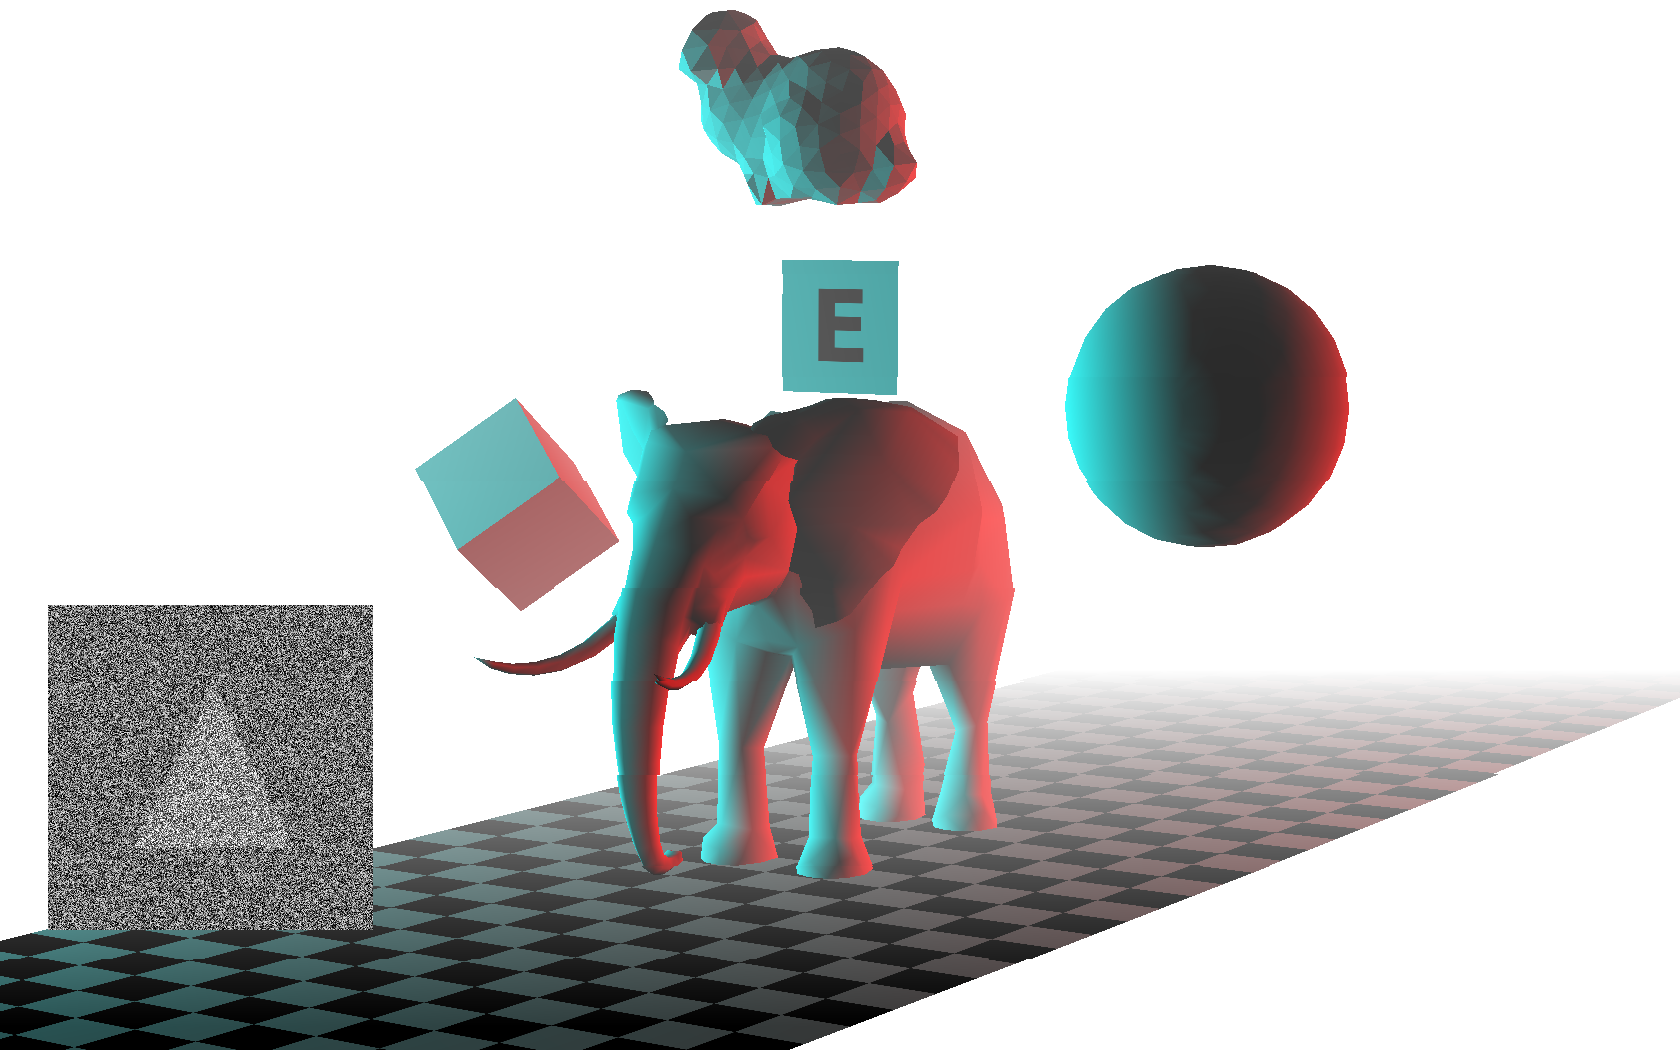
\includegraphics[width=15cm,clip,trim=0cm 0cm 0cm 0cm]{media/title.png}
\end{center}

%\begin{abstract}
%\end{abstract}

\begin{multicols}{2}

%\tableofcontents

\section{Abstract}
\paragraph{}
 \begin{abstract}
Viewing stereoscopic movies or images is unnatural. The focus and vergence of the eyes have to be decoupled. This strains the eyes, and can lead to fatigue, which makes the consumption of stereoscopic information over longer periods of times hard. But what are the physiological and psychological limits of stereoscopic viewing fatigue? And how can stereo images be composed to reduce fatigue?

Topic of this thesis is to write a Tool that enables exploration of those and similar other questions by providing a flexible and extensible framework for user testing. It is currently unclear how fatigue can be measured properly, and what scenes can be used to specifically test fatigue. Finding out which methods work and which do not is also part of this thesis.
\end{abstract}
\subsection{Stereogram\label{Stereogram}}
\paragraph{}
A stereogram is an image that contains separate data for the left and right eye. Specially crafted images can cause a binocular depth perception. The framework supports stereograms in various formats. The simplest case consists of two images, one for each eye. Several types of random dot stereograms are also available.

\subsubsection{Random dot stereogram\label{RDS}}
\paragraph{}
Random dot stereograms are a topic that has interested scientists since over a century\cite{AntRDS}. In the early 1960s they were introduced as stimuli into the modern neuroscience by Julesz\cite{BellRDS}. Unlike a normal stereogram, a RDS contains no monocular clues of the depth, or any clue about the stereoscopic image at all. This makes them the perfect tool to study binocular vision.

The two images of an RDS consist of a random pattern, usually dots. Since either image on its own is purely random, no information can be derived of it. When seen with binocular vision, depth can be seen. There are several different methods to create a random dot stereograms, but their principle is the same:
Based on depth information, parts of the pattern in one or both eyes are shifted on the horizontal axis.

\paragraph{Simple algorithm}
The first and most simple algorithm implemented is based on the original technique used by Julesz\cite{BellRDS}. A random pattern for the left eye is created, and also serves as the background in the image for the right eye. A subset of this pattern, which is defined by a mask, is shifted by a fixed amount of pixel. This is enough to create a pair of images that are on their own almost completely random, but produce a perceivable depth effect.

This approach does have problems: Areas whose contents are shifted have to be filled up again.
The chosen solution was to not move but copy the contents, so that there are duplicate patterns in the image.
Creating concave surfaces requires shifting the area in the image for the other eye, or there will be border conflicts similar to pinning.

Its advantage is that it's fast and easy to both implement and execute.
Memory access to the image buffers can be limited to one write per pixel, the pixel data for the shift can be cached in short ring buffer.

\paragraph{Advanced algorithm}
\begin{figure*}[htb]
\begin{center}
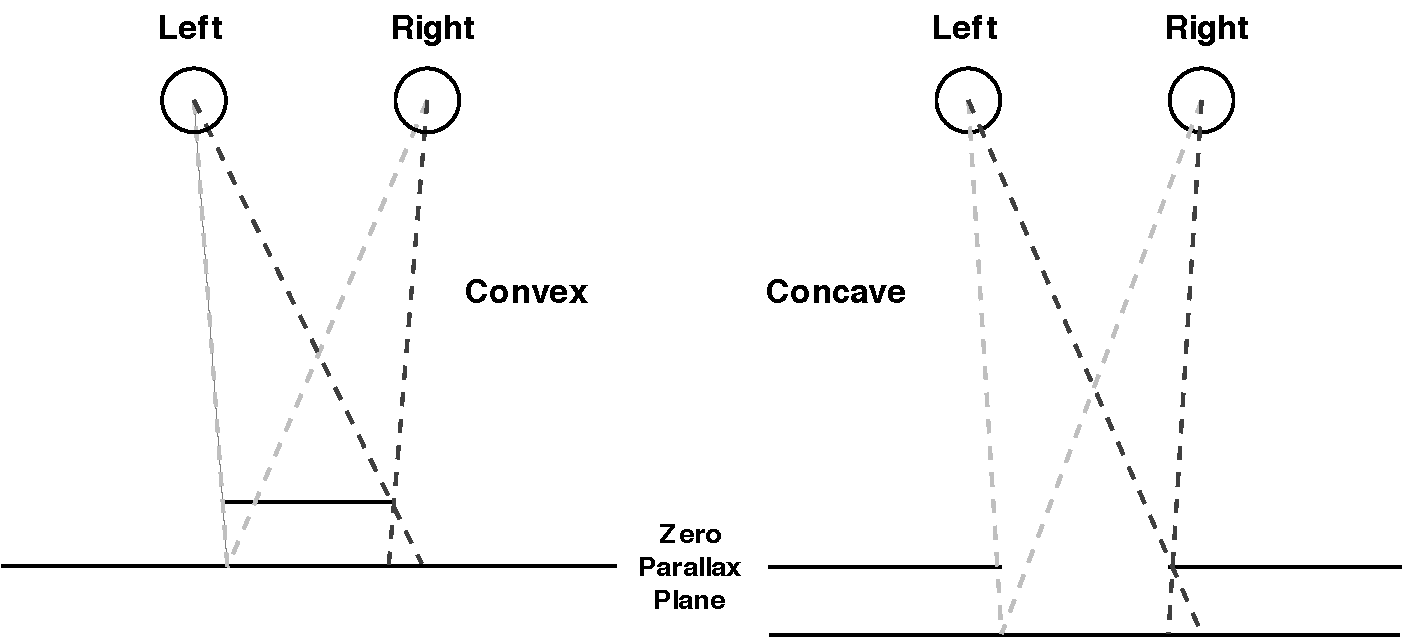
\includegraphics[width=15.5cm]{media/rds.pdf}
\caption{RDS of Convex and Concave surfaces can be created in different ways\label{ccRDS}}
\end{center}
\end{figure*}

\paragraph{}
The second algorithm is split into two parts, which deal with convex and concave stereograms separately.
This deals with subtle problems with partial occlusion (see figure \ref{ccRDS}).
It also uses different patterns for fore- and background.
Using pre-calculated patterns was loosely inspired by a paper from Gonzalez and Krause\cite{GenRDS}, which allowed different densities for object and background.

Using different colors for the foreground and the background makes the object defined in the depth map stand out. This helps visibility, but that way the shape of the object itself can not be used to validate fusion. Depending on the offset of fore- and background and the size of the random dot stereogram, it is not easily monocularly visible if the shape is convex or concave.

Both methods are simplified, the virtual cameras are always at the same relative position of the pixel in the depth map that is processed, similar to a parallel projection.

\paragraph{Convex}
The algorithm for convex shapes treats the depth map as a source to calculate the new position of pixel in a source pattern.
The calculated offset is used to displace the surface into the destination image.
The shape is shifted horizontally and appears to come out of the surface.
This is equivalent to tracking the surface of the object, and projecting the observed value onto the background (figure \ref{ccRDS}, left).
The same effect can be achieved by tracking the background, but in border cases one eye would see the background, while the other eye sees the foreground.

\paragraph{Concave}
The algorithm for concave shapes works slightly different.
It treats the depth map as a source to calculate the position of the pixel in a source pattern to place in the destination pattern.
The shape is not shifted, but its texture is.
It appears to go into the surface.
This is equivalent to tracking the background plane, and projecting the corresponding object pattern values onto the background (figure \ref{ccRDS}, right).
It can be achieved by tracking the object, but in border cases,  a point might come from the foreground for one eye, and the background for the other.

\subsubsection{Pattern stereogram}
\paragraph{}
Pattern stereograms are created similarly to random dot stereograms.
Instead of a random data source, they use a pre-computed pattern as foreground and background image.
This makes the shape stand out more and allows a high customizability of the pattern.
Possible sources include randomly generated noise images, photographed textures and randomly distributed shapes.



\end{multicols}

\appendix

\begin{thebibliography}{12}
\bibitem{AntRDS}
Bergua A., Skrandiesb W., 2000,
\textit{An early antecedent to modern random dot stereograms - 'The Secret Stereoscopic Writing' of Ram\'on y Cajal}.
Int. J. of Psychophysiology 36, 69-72\\
\url{http://dx.doi.org/10.1016/S0167-8760(99)00111-7}

\bibitem{BellRDS}
Julesz B., 1960.
\textit{Binocular depth perception of computer-generated patterns}.
Bell Syst. Tech. J. 39, 1125-1162.\\
\url{http://doi.apa.org/?uid=1961-01385-001}

\bibitem{GenRDS}
Gonzalez F., Krause F., 1994.
\textit{Generation of dynamic random-element stereograms in real time with a system based on a personal computer}.
Med. \& Biol. Eng. \& Comput., 1994, 32, 373-376.\\
\url{http://dx.doi.org/10.1007/BF02524687}

\bibitem{DepthCues}
Cutting J., Vishton P., 1995.
\textit{Perceiving layout and knowing distances: The integration, relative potency, and contextual use of different information about depth}.
In W. Epstein \& S. Rogers (Eds.), Handbook of perception and cognition, Vol. 5, 69-117. San Diego, CA: Academic Press.\\
\url{http://dx.doi.org/10.1016/B978-012240530-3/50005-5}

\end{thebibliography}

% Might only work in KOMA script (scrarticle)
\renewcommand*\refname{Links}

\begin{thebibliography}{12}
\bibitem[a]{proj} \url{http://en.wikipedia.org/wiki/Graphical_projection}
\bibitem[b]{parallel} \url{http://en.wikipedia.org/wiki/Parallel_projection}
\bibitem[c]{perspective} \url{http://en.wikipedia.org/wiki/Perspective_projection}
\bibitem[d]{painters} \url{http://en.wikipedia.org/wiki/Painter's_algorithm}
\bibitem[e]{zbuffer} \url{http://en.wikipedia.org/wiki/Z-buffering}
\bibitem[f]{fog} \url{http://www.opengl.org/documentation/specs/version1.1/glspec1.1/node90.html}
\bibitem[g]{accommodation} \url{http://en.wikipedia.org/wiki/Accommodation_(eye)}
\bibitem[h]{triangulation} \url{http://en.wikipedia.org/wiki/Triangulation}
\bibitem[i]{scenegraph} \url{http://www.realityprime.com/articles/scenegraphs-past-present-and-future}
\bibitem[j]{turing} \url{http://en.wikipedia.org/wiki/Turing_completeness}
\bibitem[k]{procedural} \url{http://en.wikipedia.org/wiki/Procedural_programming}
\end{thebibliography}




\end{document}
\end
